\documentclass[twoside]{book}

% Packages required by doxygen
\usepackage{fixltx2e}
\usepackage{calc}
\usepackage{doxygen}
\usepackage[export]{adjustbox} % also loads graphicx
\usepackage{graphicx}
\usepackage[utf8]{inputenc}
\usepackage{makeidx}
\usepackage{multicol}
\usepackage{multirow}
\PassOptionsToPackage{warn}{textcomp}
\usepackage{textcomp}
\usepackage[nointegrals]{wasysym}
\usepackage[table]{xcolor}

% Font selection
\usepackage[T1]{fontenc}
\usepackage[scaled=.90]{helvet}
\usepackage{courier}
\usepackage{amssymb}
\usepackage{sectsty}
\renewcommand{\familydefault}{\sfdefault}
\allsectionsfont{%
  \fontseries{bc}\selectfont%
  \color{darkgray}%
}
\renewcommand{\DoxyLabelFont}{%
  \fontseries{bc}\selectfont%
  \color{darkgray}%
}
\newcommand{\+}{\discretionary{\mbox{\scriptsize$\hookleftarrow$}}{}{}}

% Page & text layout
\usepackage{geometry}
\geometry{%
  a4paper,%
  top=2.5cm,%
  bottom=2.5cm,%
  left=2.5cm,%
  right=2.5cm%
}
\tolerance=750
\hfuzz=15pt
\hbadness=750
\setlength{\emergencystretch}{15pt}
\setlength{\parindent}{0cm}
\setlength{\parskip}{3ex plus 2ex minus 2ex}
\makeatletter
\renewcommand{\paragraph}{%
  \@startsection{paragraph}{4}{0ex}{-1.0ex}{1.0ex}{%
    \normalfont\normalsize\bfseries\SS@parafont%
  }%
}
\renewcommand{\subparagraph}{%
  \@startsection{subparagraph}{5}{0ex}{-1.0ex}{1.0ex}{%
    \normalfont\normalsize\bfseries\SS@subparafont%
  }%
}
\makeatother

% Headers & footers
\usepackage{fancyhdr}
\pagestyle{fancyplain}
\fancyhead[LE]{\fancyplain{}{\bfseries\thepage}}
\fancyhead[CE]{\fancyplain{}{}}
\fancyhead[RE]{\fancyplain{}{\bfseries\leftmark}}
\fancyhead[LO]{\fancyplain{}{\bfseries\rightmark}}
\fancyhead[CO]{\fancyplain{}{}}
\fancyhead[RO]{\fancyplain{}{\bfseries\thepage}}
\fancyfoot[LE]{\fancyplain{}{}}
\fancyfoot[CE]{\fancyplain{}{}}
\fancyfoot[RE]{\fancyplain{}{\bfseries\scriptsize Generated by Doxygen }}
\fancyfoot[LO]{\fancyplain{}{\bfseries\scriptsize Generated by Doxygen }}
\fancyfoot[CO]{\fancyplain{}{}}
\fancyfoot[RO]{\fancyplain{}{}}
\renewcommand{\footrulewidth}{0.4pt}
\renewcommand{\chaptermark}[1]{%
  \markboth{#1}{}%
}
\renewcommand{\sectionmark}[1]{%
  \markright{\thesection\ #1}%
}

% Indices & bibliography
\usepackage{natbib}
\usepackage[titles]{tocloft}
\setcounter{tocdepth}{3}
\setcounter{secnumdepth}{5}
\makeindex

% Hyperlinks (required, but should be loaded last)
\usepackage{ifpdf}
\ifpdf
  \usepackage[pdftex,pagebackref=true]{hyperref}
\else
  \usepackage[ps2pdf,pagebackref=true]{hyperref}
\fi
\hypersetup{%
  colorlinks=true,%
  linkcolor=blue,%
  citecolor=blue,%
  unicode%
}

% Custom commands
\newcommand{\clearemptydoublepage}{%
  \newpage{\pagestyle{empty}\cleardoublepage}%
}

\usepackage{caption}
\captionsetup{labelsep=space,justification=centering,font={bf},singlelinecheck=off,skip=4pt,position=top}

%===== C O N T E N T S =====

\begin{document}

% Titlepage & ToC
\hypersetup{pageanchor=false,
             bookmarksnumbered=true,
             pdfencoding=unicode
            }
\pagenumbering{alph}
\begin{titlepage}
\vspace*{7cm}
\begin{center}%
{\Large Employees }\\
\vspace*{1cm}
{\large Generated by Doxygen 1.8.14}\\
\end{center}
\end{titlepage}
\clearemptydoublepage
\pagenumbering{roman}
\tableofcontents
\clearemptydoublepage
\pagenumbering{arabic}
\hypersetup{pageanchor=true}

%--- Begin generated contents ---
\chapter{Hierarchical Index}
\section{Class Hierarchy}
This inheritance list is sorted roughly, but not completely, alphabetically\+:\begin{DoxyCompactList}
\item \contentsline{section}{Database\+Utils}{\pageref{class_database_utils}}{}
\item \contentsline{section}{Del\+Database\+Utils}{\pageref{class_del_database_utils}}{}
\item Q\+Dialog\begin{DoxyCompactList}
\item \contentsline{section}{Add}{\pageref{class_add}}{}
\item \contentsline{section}{Add\+Emp}{\pageref{class_add_emp}}{}
\item \contentsline{section}{Delete}{\pageref{class_delete}}{}
\item \contentsline{section}{employeeinfo}{\pageref{classemployeeinfo}}{}
\item \contentsline{section}{Search}{\pageref{class_search}}{}
\item \contentsline{section}{Update}{\pageref{class_update}}{}
\end{DoxyCompactList}
\item Q\+Main\+Window\begin{DoxyCompactList}
\item \contentsline{section}{Main\+Window}{\pageref{class_main_window}}{}
\end{DoxyCompactList}
\item \contentsline{section}{Up\+Database\+Utils}{\pageref{class_up_database_utils}}{}
\end{DoxyCompactList}

\chapter{Class Index}
\section{Class List}
Here are the classes, structs, unions and interfaces with brief descriptions\+:\begin{DoxyCompactList}
\item\contentsline{section}{\mbox{\hyperlink{class_add}{Add}} }{\pageref{class_add}}{}
\item\contentsline{section}{\mbox{\hyperlink{class_add_emp}{Add\+Emp}} }{\pageref{class_add_emp}}{}
\item\contentsline{section}{\mbox{\hyperlink{class_database_utils}{Database\+Utils}} }{\pageref{class_database_utils}}{}
\item\contentsline{section}{\mbox{\hyperlink{class_del_database_utils}{Del\+Database\+Utils}} }{\pageref{class_del_database_utils}}{}
\item\contentsline{section}{\mbox{\hyperlink{class_delete}{Delete}} }{\pageref{class_delete}}{}
\item\contentsline{section}{\mbox{\hyperlink{classemployeeinfo}{employeeinfo}} }{\pageref{classemployeeinfo}}{}
\item\contentsline{section}{\mbox{\hyperlink{class_main_window}{Main\+Window}} }{\pageref{class_main_window}}{}
\item\contentsline{section}{\mbox{\hyperlink{class_search}{Search}} }{\pageref{class_search}}{}
\item\contentsline{section}{\mbox{\hyperlink{class_up_database_utils}{Up\+Database\+Utils}} }{\pageref{class_up_database_utils}}{}
\item\contentsline{section}{\mbox{\hyperlink{class_update}{Update}} }{\pageref{class_update}}{}
\end{DoxyCompactList}

\chapter{Class Documentation}
\hypertarget{class_add}{}\section{Add Class Reference}
\label{class_add}\index{Add@{Add}}
Inheritance diagram for Add\+:\begin{figure}[H]
\begin{center}
\leavevmode
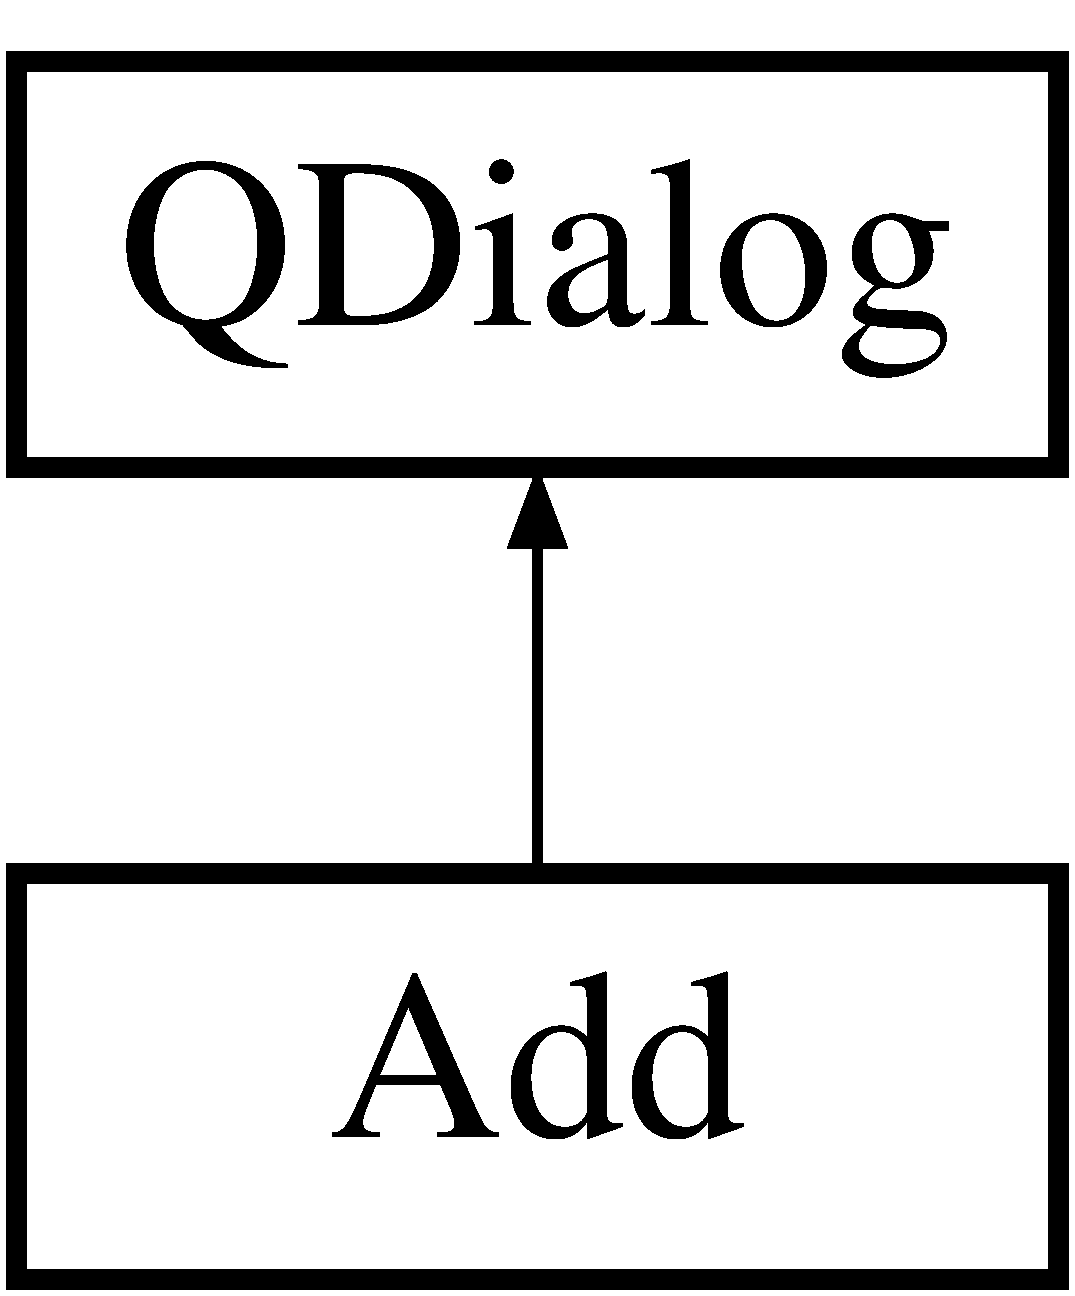
\includegraphics[height=2.000000cm]{class_add}
\end{center}
\end{figure}
\subsection*{Public Member Functions}
\begin{DoxyCompactItemize}
\item 
\mbox{\Hypertarget{class_add_a2339f812c92e0fe5341df70de15e1efe}\label{class_add_a2339f812c92e0fe5341df70de15e1efe}} 
{\bfseries Add} (Q\+Widget $\ast$parent=nullptr)
\end{DoxyCompactItemize}


The documentation for this class was generated from the following files\+:\begin{DoxyCompactItemize}
\item 
C\+:/\+Users/pc/\+Documents/\+P\+R\+O/\+E\+M\+P/add.\+h\item 
C\+:/\+Users/pc/\+Documents/\+P\+R\+O/\+E\+M\+P/add.\+cpp\end{DoxyCompactItemize}

\hypertarget{class_add_emp}{}\section{Add\+Emp Class Reference}
\label{class_add_emp}\index{Add\+Emp@{Add\+Emp}}
Inheritance diagram for Add\+Emp\+:\begin{figure}[H]
\begin{center}
\leavevmode
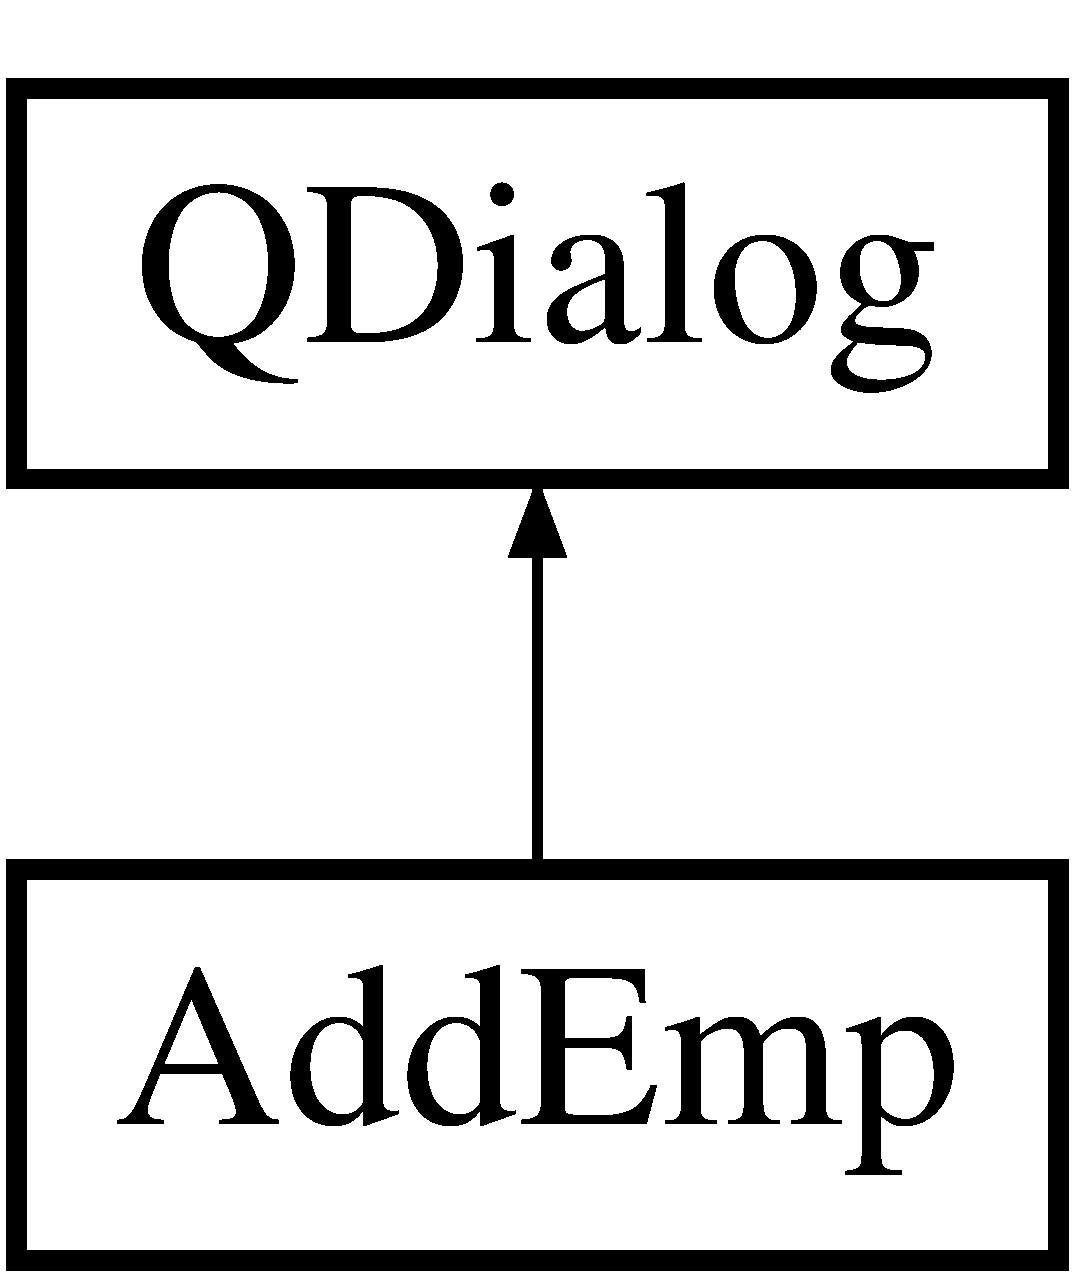
\includegraphics[height=2.000000cm]{class_add_emp}
\end{center}
\end{figure}
\subsection*{Public Member Functions}
\begin{DoxyCompactItemize}
\item 
\mbox{\Hypertarget{class_add_emp_aff93a79c68c22efe3f9074572517fdc7}\label{class_add_emp_aff93a79c68c22efe3f9074572517fdc7}} 
{\bfseries Add\+Emp} (Q\+Widget $\ast$parent=nullptr)
\end{DoxyCompactItemize}


The documentation for this class was generated from the following files\+:\begin{DoxyCompactItemize}
\item 
C\+:/\+Users/pc/\+Documents/\+P\+R\+O/\+E\+M\+P/addemp.\+h\item 
C\+:/\+Users/pc/\+Documents/\+P\+R\+O/\+E\+M\+P/addemp.\+cpp\end{DoxyCompactItemize}

\hypertarget{class_database_utils}{}\section{Database\+Utils Class Reference}
\label{class_database_utils}\index{Database\+Utils@{Database\+Utils}}
\subsection*{Public Member Functions}
\begin{DoxyCompactItemize}
\item 
\mbox{\Hypertarget{class_database_utils_ab8173fcbac13ec5f49ea319bfe5622ee}\label{class_database_utils_ab8173fcbac13ec5f49ea319bfe5622ee}} 
void {\bfseries connection\+Close} ()
\item 
\mbox{\Hypertarget{class_database_utils_a4c13f2a205cc6d07691e40c6f9c40de2}\label{class_database_utils_a4c13f2a205cc6d07691e40c6f9c40de2}} 
bool {\bfseries connection\+Open} ()
\item 
\mbox{\Hypertarget{class_database_utils_a1e86e1fff2bcf23118cbccc7561c7e77}\label{class_database_utils_a1e86e1fff2bcf23118cbccc7561c7e77}} 
Q\+Sql\+Query\+Model $\ast$ {\bfseries get\+Department\+List} ()
\item 
\mbox{\Hypertarget{class_database_utils_ad5cfa5cf873a67543730005dfd7d3d98}\label{class_database_utils_ad5cfa5cf873a67543730005dfd7d3d98}} 
Q\+Sql\+Query\+Model $\ast$ {\bfseries get\+Designation\+List} (Q\+Combo\+Box $\ast$dept)
\item 
\mbox{\Hypertarget{class_database_utils_a1cfc8637be45e2d429f0c631ce510954}\label{class_database_utils_a1cfc8637be45e2d429f0c631ce510954}} 
Q\+String {\bfseries get\+Last\+ID} ()
\item 
\mbox{\Hypertarget{class_database_utils_a9816711c985fa1aaf91ab3a3c81c441f}\label{class_database_utils_a9816711c985fa1aaf91ab3a3c81c441f}} 
Q\+String {\bfseries get\+Total\+Employee} ()
\item 
\mbox{\Hypertarget{class_database_utils_adbdfc1fd12c2eb72a4d2a7f19ff96ed5}\label{class_database_utils_adbdfc1fd12c2eb72a4d2a7f19ff96ed5}} 
Q\+String {\bfseries get\+Total\+Dept} ()
\item 
\mbox{\Hypertarget{class_database_utils_a8885c075ec313840ea820df82f639ac8}\label{class_database_utils_a8885c075ec313840ea820df82f639ac8}} 
Q\+String {\bfseries get\+Total\+Design} ()
\item 
\mbox{\Hypertarget{class_database_utils_a8c9c375135ab730563d00278fcdaa546}\label{class_database_utils_a8c9c375135ab730563d00278fcdaa546}} 
Q\+String {\bfseries get\+Employee\+ID} (Q\+String dept, Q\+String design)
\item 
\mbox{\Hypertarget{class_database_utils_a15dcd61a4107961488094c8a246cbc5b}\label{class_database_utils_a15dcd61a4107961488094c8a246cbc5b}} 
Q\+String {\bfseries get\+Designation\+Short\+Name} (Q\+Combo\+Box $\ast$design)
\item 
\mbox{\Hypertarget{class_database_utils_ae08de62e98e95d1c8b6048f8b10d2c59}\label{class_database_utils_ae08de62e98e95d1c8b6048f8b10d2c59}} 
Q\+String {\bfseries get\+Department\+Short\+Name} (Q\+Combo\+Box $\ast$dept)
\item 
\mbox{\Hypertarget{class_database_utils_ab01e50334cecf44a98cd9922d767f827}\label{class_database_utils_ab01e50334cecf44a98cd9922d767f827}} 
int {\bfseries get\+Salary} (Q\+Combo\+Box $\ast$dept, Q\+Combo\+Box $\ast$design)
\item 
\mbox{\Hypertarget{class_database_utils_af73399487169930655b66123eeb65637}\label{class_database_utils_af73399487169930655b66123eeb65637}} 
void {\bfseries set\+Employee\+Details} (Q\+Table\+View $\ast$table\+View)
\item 
\mbox{\Hypertarget{class_database_utils_aa2f3224d0bb331a5f7bed470ffcef6dd}\label{class_database_utils_aa2f3224d0bb331a5f7bed470ffcef6dd}} 
void {\bfseries search\+Employee\+Details} (Q\+Table\+View $\ast$search\+Table\+View, Q\+String search\+Text)
\item 
\mbox{\Hypertarget{class_database_utils_a915e1d43584500e2519f67265b0d792f}\label{class_database_utils_a915e1d43584500e2519f67265b0d792f}} 
void {\bfseries set\+Employee\+Update\+Details} (Q\+Table\+View $\ast$Uptable\+View)
\item 
\mbox{\Hypertarget{class_database_utils_a9ef5766e143076e2334495282706b9c3}\label{class_database_utils_a9ef5766e143076e2334495282706b9c3}} 
Q\+Sql\+Query $\ast$ {\bfseries show\+Employee\+Details\+To\+Line\+Edit} (Q\+String id)
\item 
\mbox{\Hypertarget{class_database_utils_a15083ce47b8e821f13e6884c8bb3666c}\label{class_database_utils_a15083ce47b8e821f13e6884c8bb3666c}} 
void {\bfseries delete\+Employee\+Record} (Q\+String id)
\end{DoxyCompactItemize}
\subsection*{Public Attributes}
\begin{DoxyCompactItemize}
\item 
\mbox{\Hypertarget{class_database_utils_ad6b57582f89ccd499b7653f2f1912654}\label{class_database_utils_ad6b57582f89ccd499b7653f2f1912654}} 
Q\+Sql\+Database {\bfseries Employ}
\end{DoxyCompactItemize}


The documentation for this class was generated from the following file\+:\begin{DoxyCompactItemize}
\item 
C\+:/\+Users/pc/\+Documents/\+P\+R\+O/\+E\+M\+P/databaseutils.\+cpp\end{DoxyCompactItemize}

\hypertarget{class_del_database_utils}{}\section{Del\+Database\+Utils Class Reference}
\label{class_del_database_utils}\index{Del\+Database\+Utils@{Del\+Database\+Utils}}
\subsection*{Public Member Functions}
\begin{DoxyCompactItemize}
\item 
\mbox{\Hypertarget{class_del_database_utils_ad4a80936857bfb7f53a06e5f3ce4627c}\label{class_del_database_utils_ad4a80936857bfb7f53a06e5f3ce4627c}} 
void {\bfseries connection\+Close} ()
\item 
\mbox{\Hypertarget{class_del_database_utils_a8a7064a79b1d6067f26c1fc5859e0072}\label{class_del_database_utils_a8a7064a79b1d6067f26c1fc5859e0072}} 
bool {\bfseries connection\+Open} ()
\item 
\mbox{\Hypertarget{class_del_database_utils_ae4e210daae25b32f7243d8dba2d6537c}\label{class_del_database_utils_ae4e210daae25b32f7243d8dba2d6537c}} 
void {\bfseries delete\+Employee\+Record} (Q\+String id)
\end{DoxyCompactItemize}
\subsection*{Public Attributes}
\begin{DoxyCompactItemize}
\item 
\mbox{\Hypertarget{class_del_database_utils_ab9b1cdf9ab3707f14c578892f1da9c0c}\label{class_del_database_utils_ab9b1cdf9ab3707f14c578892f1da9c0c}} 
Q\+Sql\+Database {\bfseries Employ}
\end{DoxyCompactItemize}


The documentation for this class was generated from the following file\+:\begin{DoxyCompactItemize}
\item 
C\+:/\+Users/pc/\+Documents/\+P\+R\+O/\+E\+M\+P/deldatabaseutils.\+cpp\end{DoxyCompactItemize}

\hypertarget{class_delete}{}\section{Delete Class Reference}
\label{class_delete}\index{Delete@{Delete}}
Inheritance diagram for Delete\+:\begin{figure}[H]
\begin{center}
\leavevmode
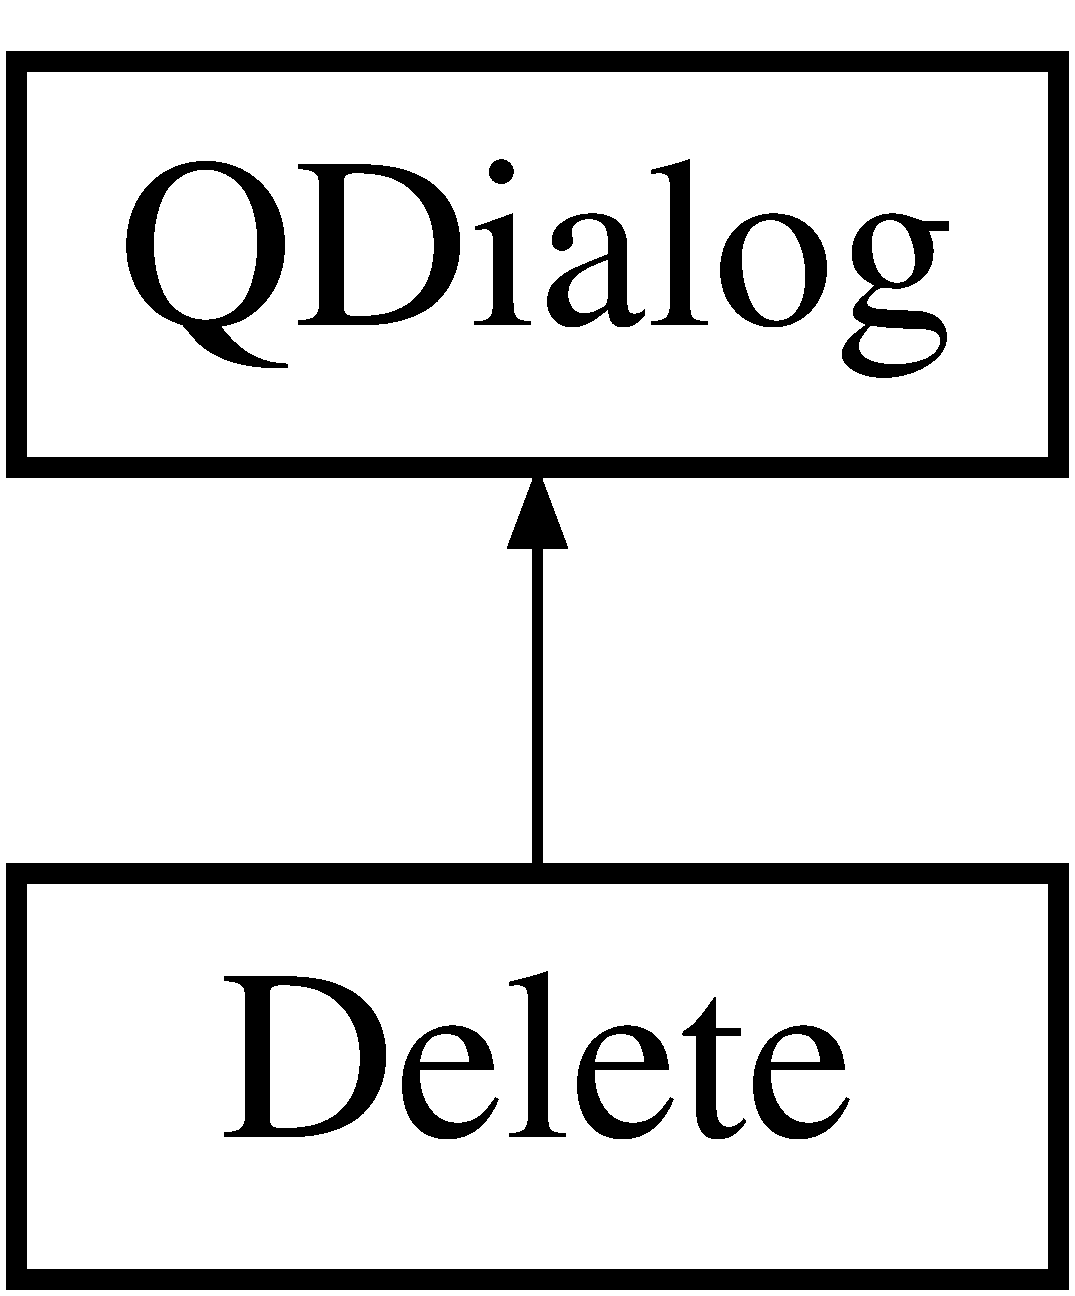
\includegraphics[height=2.000000cm]{class_delete}
\end{center}
\end{figure}
\subsection*{Public Member Functions}
\begin{DoxyCompactItemize}
\item 
\mbox{\Hypertarget{class_delete_a6ff051994905bc978e3a9e53bb48145e}\label{class_delete_a6ff051994905bc978e3a9e53bb48145e}} 
{\bfseries Delete} (Q\+Widget $\ast$parent=nullptr)
\end{DoxyCompactItemize}
\subsection*{Public Attributes}
\begin{DoxyCompactItemize}
\item 
\mbox{\Hypertarget{class_delete_a01d3766e364970e9adb7d96e539ea5b3}\label{class_delete_a01d3766e364970e9adb7d96e539ea5b3}} 
\mbox{\hyperlink{class_del_database_utils}{Del\+Database\+Utils}} {\bfseries Utils}
\end{DoxyCompactItemize}


The documentation for this class was generated from the following files\+:\begin{DoxyCompactItemize}
\item 
C\+:/\+Users/pc/\+Documents/\+P\+R\+O/\+E\+M\+P/delete.\+h\item 
C\+:/\+Users/pc/\+Documents/\+P\+R\+O/\+E\+M\+P/delete.\+cpp\end{DoxyCompactItemize}

\hypertarget{classemployeeinfo}{}\section{employeeinfo Class Reference}
\label{classemployeeinfo}\index{employeeinfo@{employeeinfo}}
Inheritance diagram for employeeinfo\+:\begin{figure}[H]
\begin{center}
\leavevmode
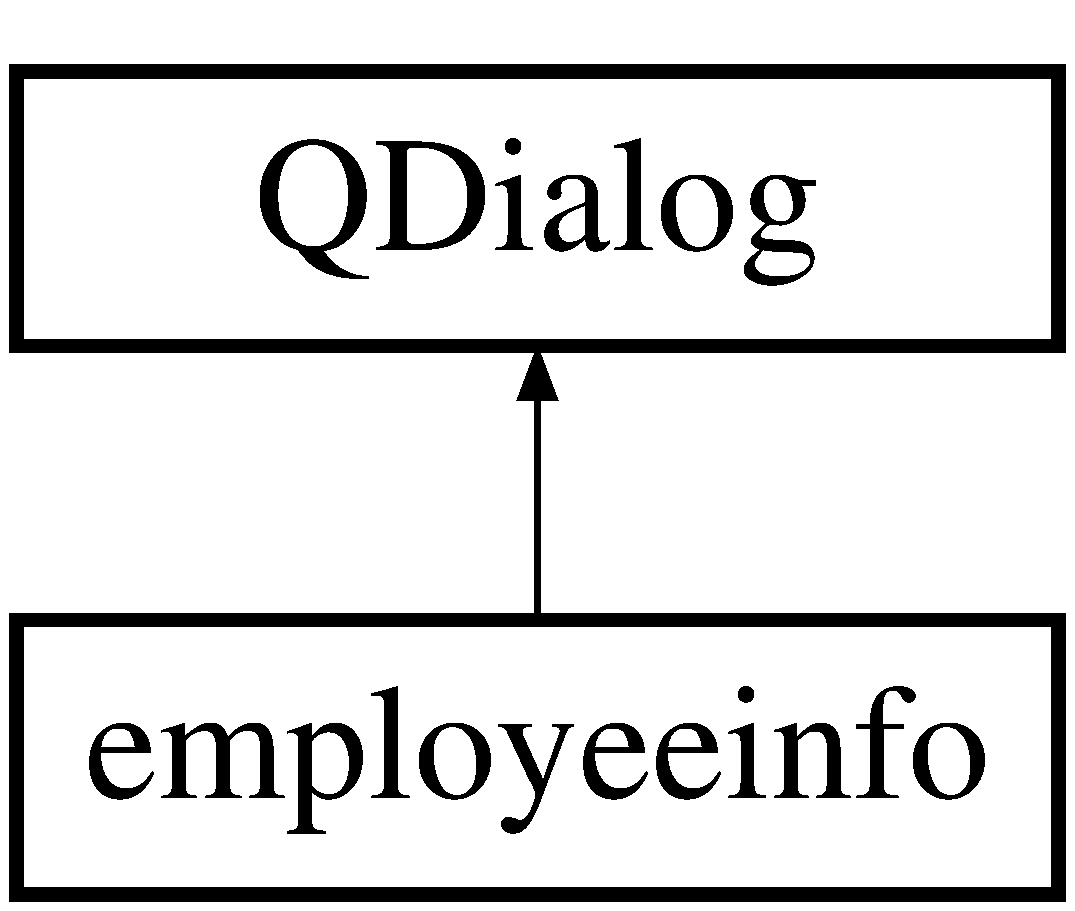
\includegraphics[height=2.000000cm]{classemployeeinfo}
\end{center}
\end{figure}
\subsection*{Public Member Functions}
\begin{DoxyCompactItemize}
\item 
\mbox{\Hypertarget{classemployeeinfo_a309c67c5a4eebc1008c877df78551f9a}\label{classemployeeinfo_a309c67c5a4eebc1008c877df78551f9a}} 
{\bfseries employeeinfo} (Q\+Widget $\ast$parent=nullptr)
\end{DoxyCompactItemize}


The documentation for this class was generated from the following file\+:\begin{DoxyCompactItemize}
\item 
C\+:/\+Users/pc/\+Documents/\+P\+R\+O/\+E\+M\+P/employeeinfo.\+h\end{DoxyCompactItemize}

\hypertarget{class_main_window}{}\section{Main\+Window Class Reference}
\label{class_main_window}\index{Main\+Window@{Main\+Window}}
Inheritance diagram for Main\+Window\+:\begin{figure}[H]
\begin{center}
\leavevmode
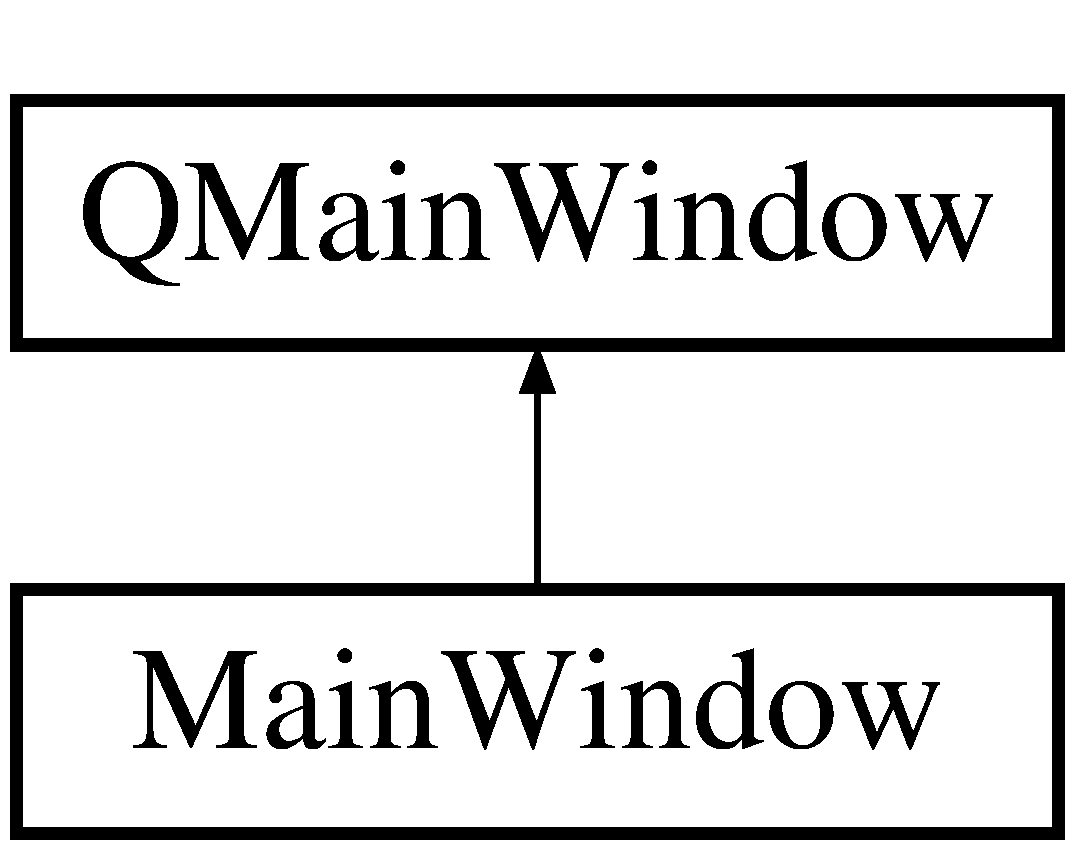
\includegraphics[height=2.000000cm]{class_main_window}
\end{center}
\end{figure}
\subsection*{Public Member Functions}
\begin{DoxyCompactItemize}
\item 
\mbox{\Hypertarget{class_main_window_a57019e6e2280b38e01d682512a33fb91}\label{class_main_window_a57019e6e2280b38e01d682512a33fb91}} 
void {\bfseries connection\+Close} ()
\item 
\mbox{\Hypertarget{class_main_window_a1c01c05ca5290d3920ce01b69ad6f69d}\label{class_main_window_a1c01c05ca5290d3920ce01b69ad6f69d}} 
bool {\bfseries connection\+Open} ()
\item 
\mbox{\Hypertarget{class_main_window_a996c5a2b6f77944776856f08ec30858d}\label{class_main_window_a996c5a2b6f77944776856f08ec30858d}} 
{\bfseries Main\+Window} (Q\+Widget $\ast$parent=nullptr)
\end{DoxyCompactItemize}
\subsection*{Public Attributes}
\begin{DoxyCompactItemize}
\item 
\mbox{\Hypertarget{class_main_window_afb299526cf3286937e7c11c3c5f21c0d}\label{class_main_window_afb299526cf3286937e7c11c3c5f21c0d}} 
Q\+Sql\+Database {\bfseries Employ}
\end{DoxyCompactItemize}


The documentation for this class was generated from the following files\+:\begin{DoxyCompactItemize}
\item 
C\+:/\+Users/pc/\+Documents/\+P\+R\+O/\+E\+M\+P/mainwindow.\+h\item 
C\+:/\+Users/pc/\+Documents/\+P\+R\+O/\+E\+M\+P/mainwindow.\+cpp\end{DoxyCompactItemize}

\hypertarget{class_search}{}\section{Search Class Reference}
\label{class_search}\index{Search@{Search}}
Inheritance diagram for Search\+:\begin{figure}[H]
\begin{center}
\leavevmode
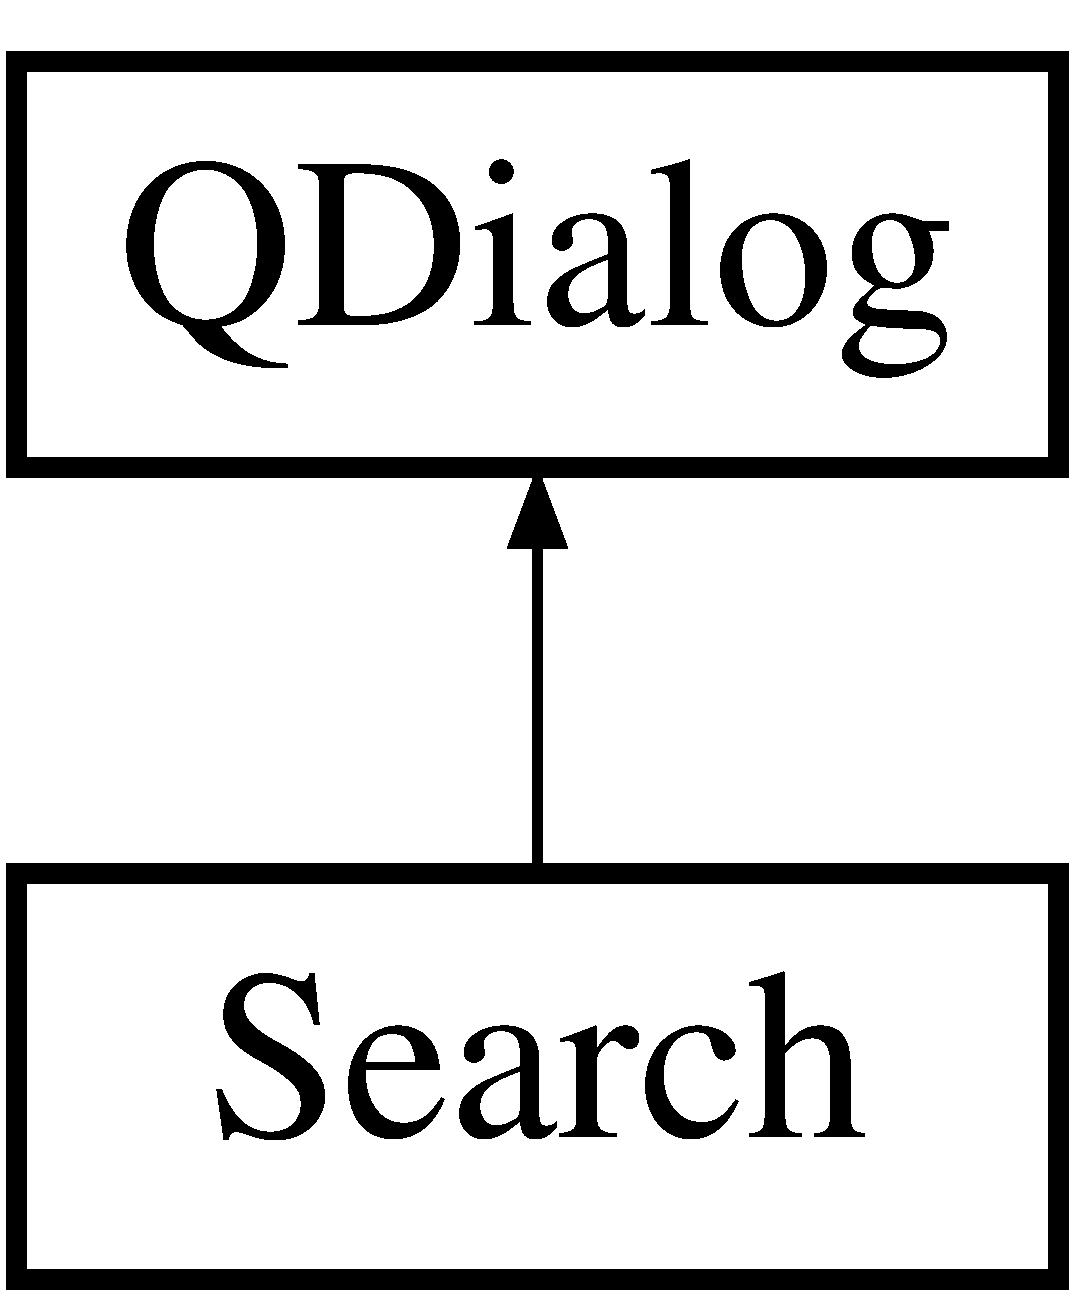
\includegraphics[height=2.000000cm]{class_search}
\end{center}
\end{figure}
\subsection*{Public Member Functions}
\begin{DoxyCompactItemize}
\item 
\mbox{\Hypertarget{class_search_a7010bf2c93cc36c96a19ae568a58fb28}\label{class_search_a7010bf2c93cc36c96a19ae568a58fb28}} 
{\bfseries Search} (Q\+Widget $\ast$parent=nullptr)
\end{DoxyCompactItemize}
\subsection*{Public Attributes}
\begin{DoxyCompactItemize}
\item 
\mbox{\Hypertarget{class_search_ae15bf78c3cb5b09062d436929ce82d5b}\label{class_search_ae15bf78c3cb5b09062d436929ce82d5b}} 
\mbox{\hyperlink{class_database_utils}{Database\+Utils}} {\bfseries db\+Utils}
\end{DoxyCompactItemize}


The documentation for this class was generated from the following files\+:\begin{DoxyCompactItemize}
\item 
C\+:/\+Users/pc/\+Documents/\+P\+R\+O/\+E\+M\+P/search.\+h\item 
C\+:/\+Users/pc/\+Documents/\+P\+R\+O/\+E\+M\+P/search.\+cpp\end{DoxyCompactItemize}

\hypertarget{class_up_database_utils}{}\section{Up\+Database\+Utils Class Reference}
\label{class_up_database_utils}\index{Up\+Database\+Utils@{Up\+Database\+Utils}}
\subsection*{Public Member Functions}
\begin{DoxyCompactItemize}
\item 
\mbox{\Hypertarget{class_up_database_utils_a68c2dcea1af63cdb9c76449eb89204ec}\label{class_up_database_utils_a68c2dcea1af63cdb9c76449eb89204ec}} 
void {\bfseries connection\+Close} ()
\item 
\mbox{\Hypertarget{class_up_database_utils_ac3e40dec44baf833c156920eebff6860}\label{class_up_database_utils_ac3e40dec44baf833c156920eebff6860}} 
bool {\bfseries connection\+Open} ()
\item 
\mbox{\Hypertarget{class_up_database_utils_a3fd9951060f82141ac0b7096b2be330c}\label{class_up_database_utils_a3fd9951060f82141ac0b7096b2be330c}} 
void {\bfseries set\+Employee\+Update\+Details} (Q\+Table\+View $\ast$Uptable\+View)
\item 
\mbox{\Hypertarget{class_up_database_utils_a21b16b7d0f438d1535f45b23ea5901dd}\label{class_up_database_utils_a21b16b7d0f438d1535f45b23ea5901dd}} 
Q\+Sql\+Query $\ast$ {\bfseries show\+Employee\+Details\+To\+Line\+Edit} (Q\+String id)
\end{DoxyCompactItemize}
\subsection*{Public Attributes}
\begin{DoxyCompactItemize}
\item 
\mbox{\Hypertarget{class_up_database_utils_a7729ca29a54ab9865dac411503c3d5b3}\label{class_up_database_utils_a7729ca29a54ab9865dac411503c3d5b3}} 
Q\+Sql\+Database {\bfseries Employ}
\end{DoxyCompactItemize}


The documentation for this class was generated from the following file\+:\begin{DoxyCompactItemize}
\item 
C\+:/\+Users/pc/\+Documents/\+P\+R\+O/\+E\+M\+P/updatabaseutils.\+cpp\end{DoxyCompactItemize}

\hypertarget{class_update}{}\section{Update Class Reference}
\label{class_update}\index{Update@{Update}}
Inheritance diagram for Update\+:\begin{figure}[H]
\begin{center}
\leavevmode
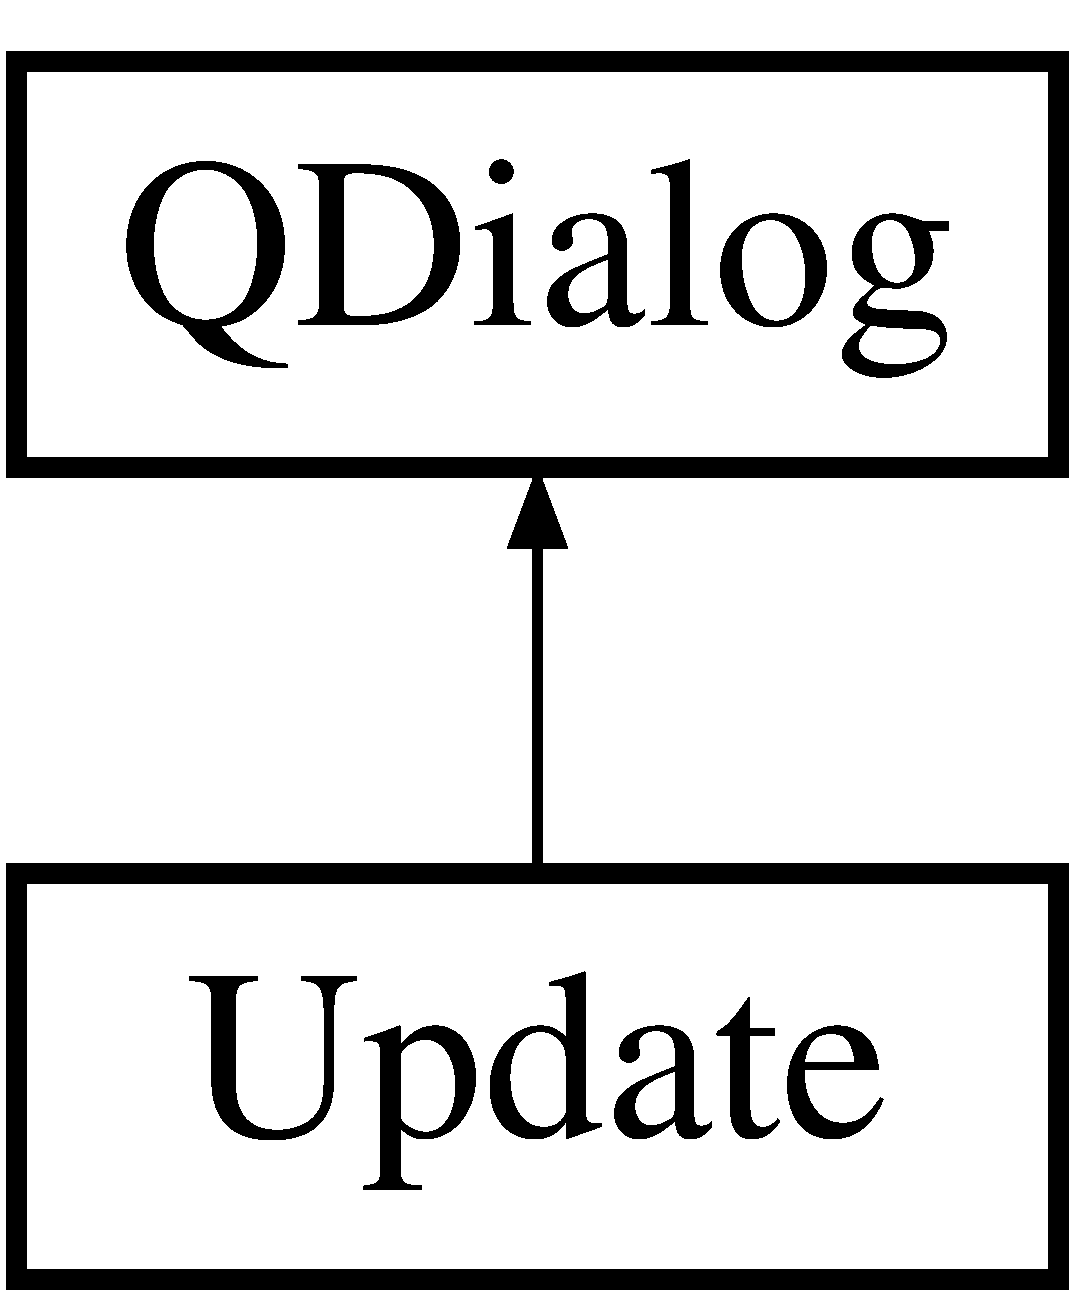
\includegraphics[height=2.000000cm]{class_update}
\end{center}
\end{figure}
\subsection*{Public Member Functions}
\begin{DoxyCompactItemize}
\item 
\mbox{\Hypertarget{class_update_aa4739ce246ffdcbe087f76f7d19af197}\label{class_update_aa4739ce246ffdcbe087f76f7d19af197}} 
{\bfseries Update} (Q\+Widget $\ast$parent=nullptr)
\end{DoxyCompactItemize}
\subsection*{Public Attributes}
\begin{DoxyCompactItemize}
\item 
\mbox{\Hypertarget{class_update_a4545f0eb2b60ec434ee9d0b5448f7c4f}\label{class_update_a4545f0eb2b60ec434ee9d0b5448f7c4f}} 
\mbox{\hyperlink{class_up_database_utils}{Up\+Database\+Utils}} {\bfseries d\+Utils}
\end{DoxyCompactItemize}


The documentation for this class was generated from the following files\+:\begin{DoxyCompactItemize}
\item 
C\+:/\+Users/pc/\+Documents/\+P\+R\+O/\+E\+M\+P/update.\+h\item 
C\+:/\+Users/pc/\+Documents/\+P\+R\+O/\+E\+M\+P/update.\+cpp\end{DoxyCompactItemize}

%--- End generated contents ---

% Index
\backmatter
\newpage
\phantomsection
\clearemptydoublepage
\addcontentsline{toc}{chapter}{Index}
\printindex

\end{document}
